\documentclass{beamer}


\mode<presentation>
{
  \usetheme{CambridgeUS}
	\usecolortheme{beaver}
  % or ...

  \setbeamercovered{transparent}
  % or whatever (possibly just delete it)
}


\usepackage{xeCJK}
\usepackage{ulem}
\usepackage[english]{babel}
\usepackage[utf8]{inputenc}
\usepackage{times}
\usepackage[T1]{fontenc}
\usepackage{hyperref}
\usepackage{pifont}
\usepackage{biblatex}
\usepackage{bibentry}
\usepackage{verbatim}
\bibliography{cite}
\newcommand{\cmark}{\ding{51}}%
\newcommand{\xmark}{\ding{55}}%
\setCJKmainfont{WenQuanYi Micro Hei}
\renewcommand{\raggedright}{\leftskip=0pt \rightskip=0pt plus 0cm}
\raggedright

\let\oldfootnotesize\footnotesize
\renewcommand*{\footnotesize}{\oldfootnotesize\tiny}

\title[Games and Software Engineering] 
{Games and Software Engineering}
\subtitle{NetHack}

\author[Zhilei Ren] 
{Zhilei Ren}

\institute[OSCAR Team] % (optional, but mostly needed)
{
\\
\includegraphics[width=0.2\textwidth]{../../utils/logo.jpg}\\
OSCAR Team, School of Software, 
Dalian University of Technology
}


\subject{Open Source}



\pgfdeclareimage[height=0.5cm]{university-logo}{../../utils/logo.jpg}
\logo{\pgfuseimage{university-logo}}



% Delete this, if you do not want the table of contents to pop up at
% the beginning of each subsection:
\AtBeginSubsection[]
{
  \begin{frame}<beamer>{Outline}
    \tableofcontents[currentsection,currentsubsection]
  \end{frame}
}


% If you wish to uncover everything in a step-wise fashion, uncomment
% the following command: 

%\beamerdefaultoverlayspecification{<+->}

\setbeamertemplate{section in toc}[circle]
\setbeamertemplate{items}[circle]
\setbeamertemplate{caption}[numbered]
\setbeamertemplate{bibliography item}{\insertbiblabel}
\setbeamertemplate{bibliography entry title}{}
\setbeamertemplate{bibliography entry journal}{}

\begin{document}

\begin{frame}
  \titlepage
\end{frame}

%\begin{frame}{Outline}
%  \tableofcontents[currentsection,currentsubsection, 
%    hideothersubsections, 
%    sectionstyle=show,
%]
%\end{frame}

\AtBeginSection[]
{
 \begin{frame}<beamer>
 \frametitle{Outline}
 \tableofcontents[currentsection]
 \end{frame}
}
\begin{frame}[t]{Rogue}

    Rogue是迷宫探索式电子游戏，最早由迈克尔·托依和格伦·韦科曼在1980年左右开发\footnote{\url{https://zh.wikipedia.org/wiki/Rogue}}。部分因为游戏内容的过程生成，游戏在1980年代中期大学Unix系统上很流行。Rogue使迷宫探索在电子游戏领域普及，其他开发者制作了诸多统称为“类rogue”（Roguelike）的派生作品。比如它直接给与了Hack灵感，此游戏之后又衍生出NetHack。类rogue还影响了其他类型的商业游戏，如暗黑破坏神
    Rogue在当时的计算机研究者和大学生之间引发轰动，甚至Unix之父之一的肯·汤普逊也沉迷其中。丹尼斯·里奇开玩笑道：“Rogue就是史上最浪费CPU时钟周期的东西（the biggest waste of CPU cycles in history）”
\end{frame}

\begin{frame}[t]{RogueLike}
    游戏玩法核心元素在2008年的柏林国际Roguelike游戏开发大会得到了明确的定义，称之为“柏林准则”
    \begin{itemize}
        \item 通过随机生成地牢来增强可玩性 
        \item 游戏使用永久死亡机制
        \item 游戏是回合制的
        \item 游戏不应该有过多限制
        \item 游戏应该为玩家提供完成同样方式的多种不同方法
        \item 为了生存玩家必须妥善管理自己的资源
        \item 游戏核心内容应是hack and slash
        \item 游戏要求玩家探索地图，寻找宝藏并杜绝背板
    \end{itemize}
\end{frame}

\begin{frame}[t]{Hack and NetHack}
    Hack（1982年）是杰·芬拉森（Jay Fenlason）在肯尼·伍德蓝德（Kenny Woodland）、麦克·托米（Mike Thome）和强纳森·沛恩（Jonathan Payne）的帮助下开发的。他们曾找到Rogue的制作者托伊和阿诺，希望能获取游戏源代码，却遭到拒绝，这迫使他们从原有的游戏草稿设计一个完整的游戏出来。

麦克·史蒂芬森（Mike Stephenson）接手Hack的代码维护工作后，他按照美国宾夕法尼亚大学哲学教授伊兹查克·米勒和电脑极客珍妮特·瓦兹（Janet Walz）的建议改进了这款游戏。这三位组建了一个“开发组”，着手对Hack的源代码做重大修改。部分因为他们的工作主要通过USENET来沟通，他们称修改后的版本为NetHack，Net便是指该游戏通过网络开发。
\end{frame}

\begin{frame}[t]{NetHack}

    \begin{itemize}
        \item NetHack是一款最初在1987年发布的Roguelike单人游戏，拥有由ASCII字符组成的图形界面。它继承了Hack（1985年）及更早的Rogue（1980年）。\footnote{\url{https://zh.wikipedia.org/wiki/NetHack}}
        \item 游戏名字中的“网络”（Net）是指开发过程通过互联网合作完成。
        \item 而“Hack”是指角色扮演游戏的特点——hack and slash。
        \item 玩家扮演一个地下城探险者寻找Yendor的项链。
        \item 玩家需要选择自己所扮演的角色并指定性别、种族、职业和阵营，或者选择让系统随机产生一个角色。游戏者可以扮演经典奇幻角色，比如骑士、野蛮人、巫师、游侠、女武神、僧侣和武士，也可以选择一些比较少见的角色，诸如考古学家、游客和洞穴人。
    \end{itemize}
\end{frame}

\begin{frame}[t]{Nethack}
    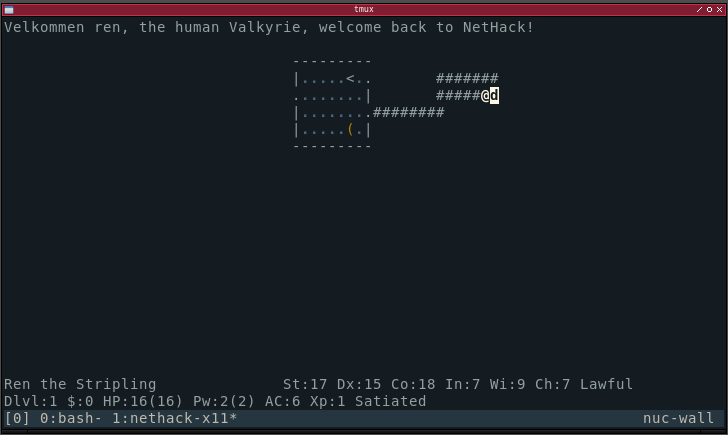
\includegraphics[height=.25\textwidth]{nethack.png} 
    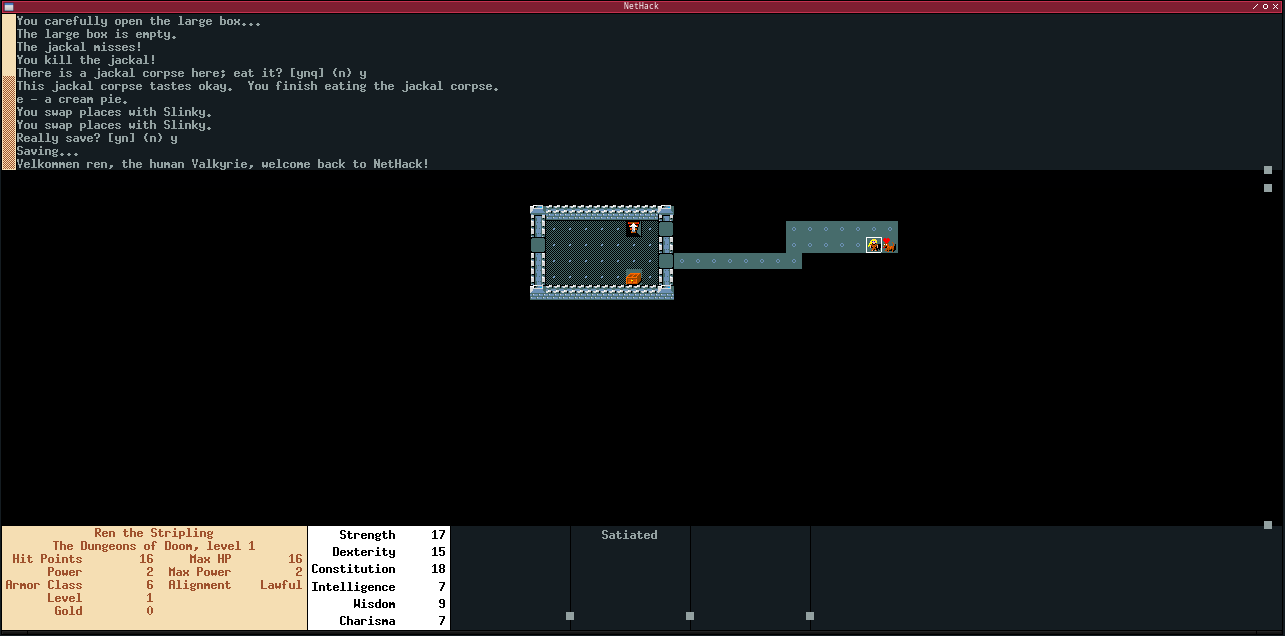
\includegraphics[height=.25\textwidth]{xnethack.png} 
    \\
    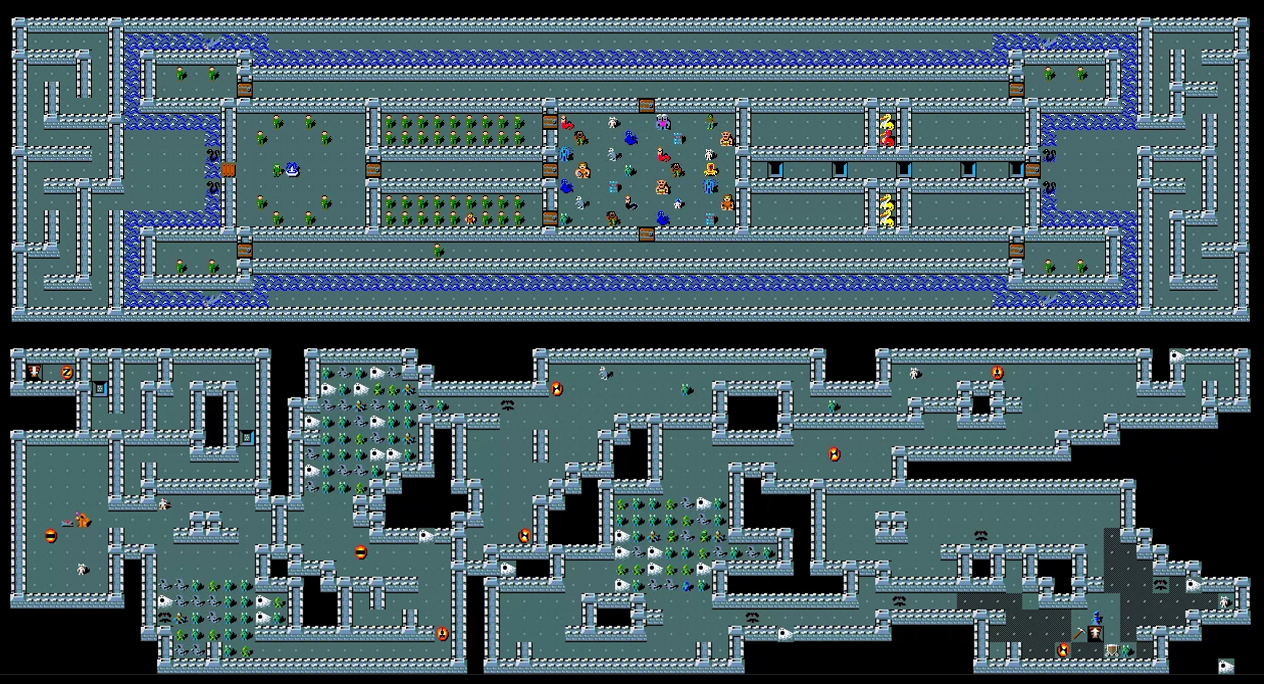
\includegraphics[width=.5\textwidth]{level_crop.png} 

\end{frame}
\begin{frame}[t]{NetHack Learning Environment}
    Facebook artificial intelligence (AI) research， University of Oxford, New York University，Imperial College London，University College London开发了一个基于NetHack的学习环境NetHack Learning Environment

    2021 Conference on Neural Information Processing Systems组织了竞赛，但无人完赛，排名第一使用符号推理而非神经网络
\end{frame}

\end{document}

